\documentclass[a4paper,12pt]{article}
\usepackage{mathtools}
\usepackage {amsmath}
\usepackage{graphicx}
\usepackage[section]{placeins}
\usepackage{caption}
\usepackage{subcaption}
\usepackage{float}
\usepackage[a4paper, total={6.5in, 10in}]{geometry}
\usepackage{times}
\usepackage{gensymb}
\usepackage[document]{ragged2e}

\title{CSC 22100: Exercise 3}

%%% BEGIN DOCUMENT
\begin{document}

\newpage
\maketitle
\tableofcontents

\pagebreak
\listoffigures

\newpage


\section{Part 1}

\subsection{Instructions}
Implement a Java class PieChart that displays a pie chart of the probabilities of the n most frequent occurrences of an event to be specified in part 3 of the exercise. The probability of event is given by the equation:


\begin{equation} \label{ProbabilityEquation}
Probability \ of \ event = \frac{Frequency \ of  \ event}{\Sigma Frequencies  \ of \ all \ events}
\end{equation}


In the pie chart: \newline

i. The area of each segment is proportional to the probability of the corresponding event:

\begin{equation}  \label{equationForAngles}
Probability \ of \ event = \frac{Central \ angle \ of \ segment}{2 \pi }
\end{equation}



ii. Each segment has a different color;	

iii. Each segment has a legend showing the event and its probability; \newline
iv. The last segment represents ?All Other Events? and their cumulative
probability. For example, in the graph below where the event is the occurrence of a letter in a text: n = 3, and the probability of All Other Events is one minus the sum of the probabilities of events e, s, and i;

\begin{figure}[H]
   \centering
   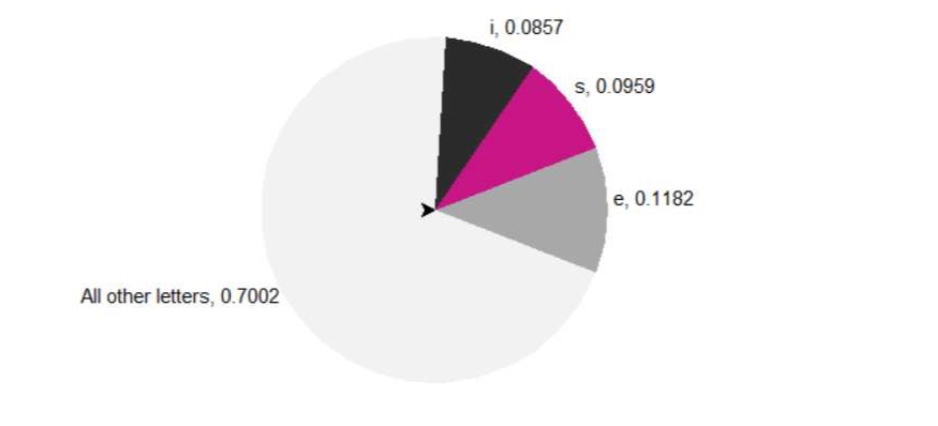
\includegraphics[width = 17cm]{pieChartExample} % requires the graphicx package
   \caption{ShapePositionInterface Part2}
   \label{ShapePositionInterface Part2}
\end{figure}

\subsection{Solution Method}

The implementation for the PieChart class is shown in figures \ref{pieChartPart1} to \ref{pieChartPart4}. Lines 6 - 17 the private members n, probabilityOfEvents, centralAngleOfSegments, typesOfEvents, and colorList are declared. n refers to the number of different events that the pie chart will include,  probabilityOfEvents is an array of doubles containing the probability for each event as defined in equation \ref{ProbabilityEquation}, and centralAngleOfSegments is an array containing the angles which will be used to draw the pie chart. typesOfEvents is the array containing the different events will might occur, in the case of the Histogram, it includes the 26 letters of the english alphabet.  \newline

\vspace{0.25cm}
It is important to realize that the PieChart class extends the class Circle, which extends the class Shape. That's why in the constructor in lines 20 - 26 the keyword super is used to properly initiate the member variables of its superclasses. Method calculateCentralAngleOfSegment() is included in lines 28 - 34, this uses the equation \ref{equationForAngles} to calculate the angle of each event.  \newline

\vspace{0.25cm}
Finally, the draw() and addLegend() methods were implemented in lines 36 - 66, and 68 - 118, respectively. 
The draw method starts by calling the method calculateCentralAngleOfSegment  to calculate the angles for each event. First, a for loop draw the arcs for the first 20th most frequent letters with different colors. The six less frequent letters are all drawn with the same color to avoid crowding the legends on the pie chart drawing. The addLegend() process all the events in a similar fashion than the draw method. This however uses a set of if - else statements to properly locate the place of the legends regarding their quadrant on the canvas. At the end of the PieChar class, a sort method is included which was used to sort the probabilities of letters in decreasing order.

\subsection{Code Developed}


\begin{figure}[H]
   \centering
   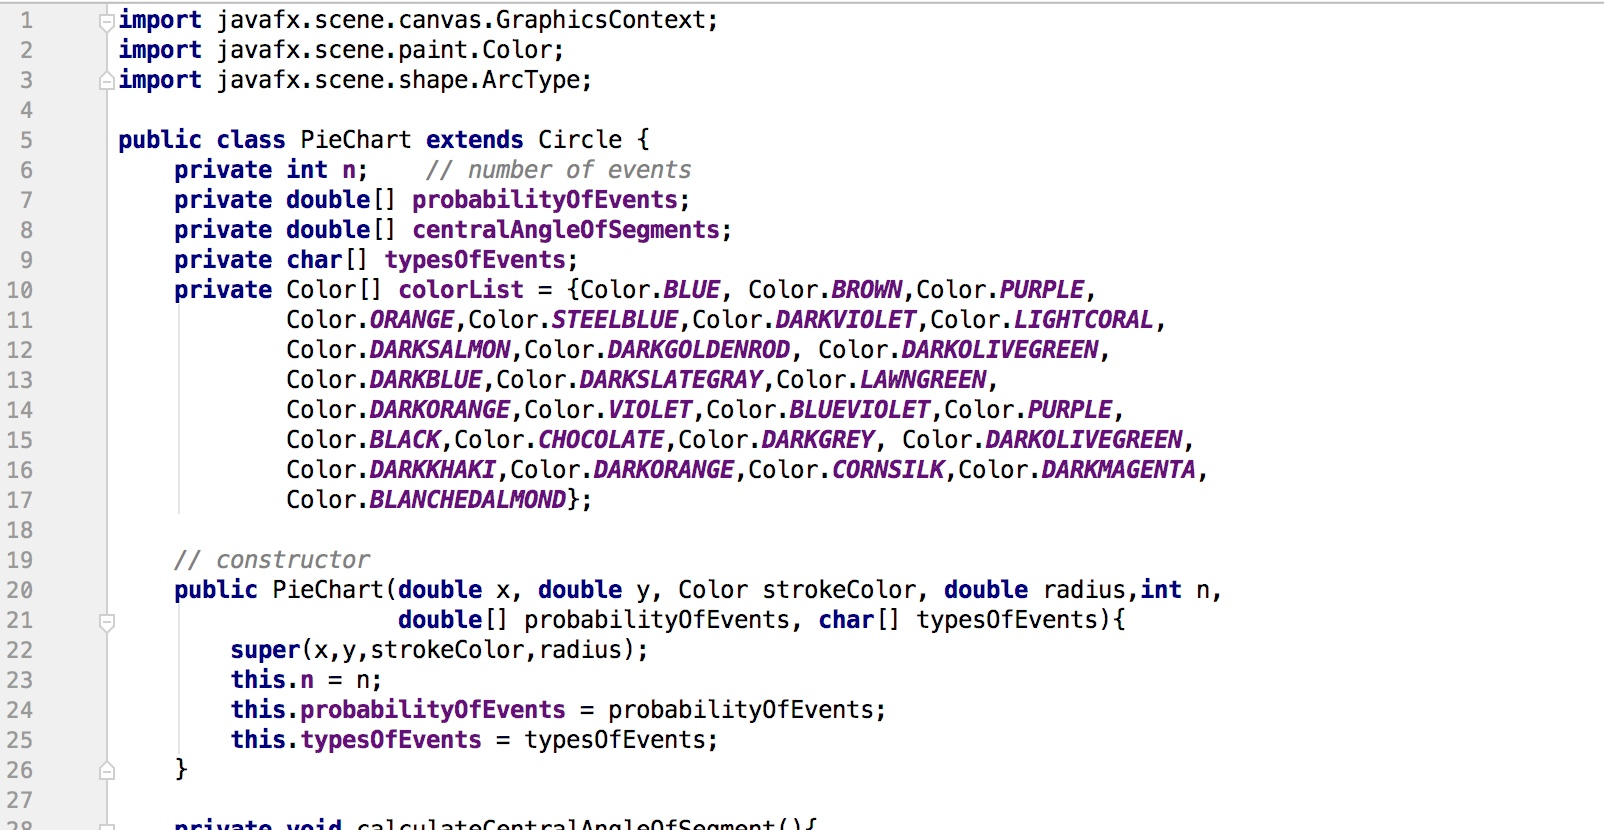
\includegraphics[width = 17cm]{pieChartPart1} % requires the graphicx package
   \caption{pieChartPart1}
   \label{pieChartPart1}
\end{figure}



\begin{figure}[H]
   \centering
   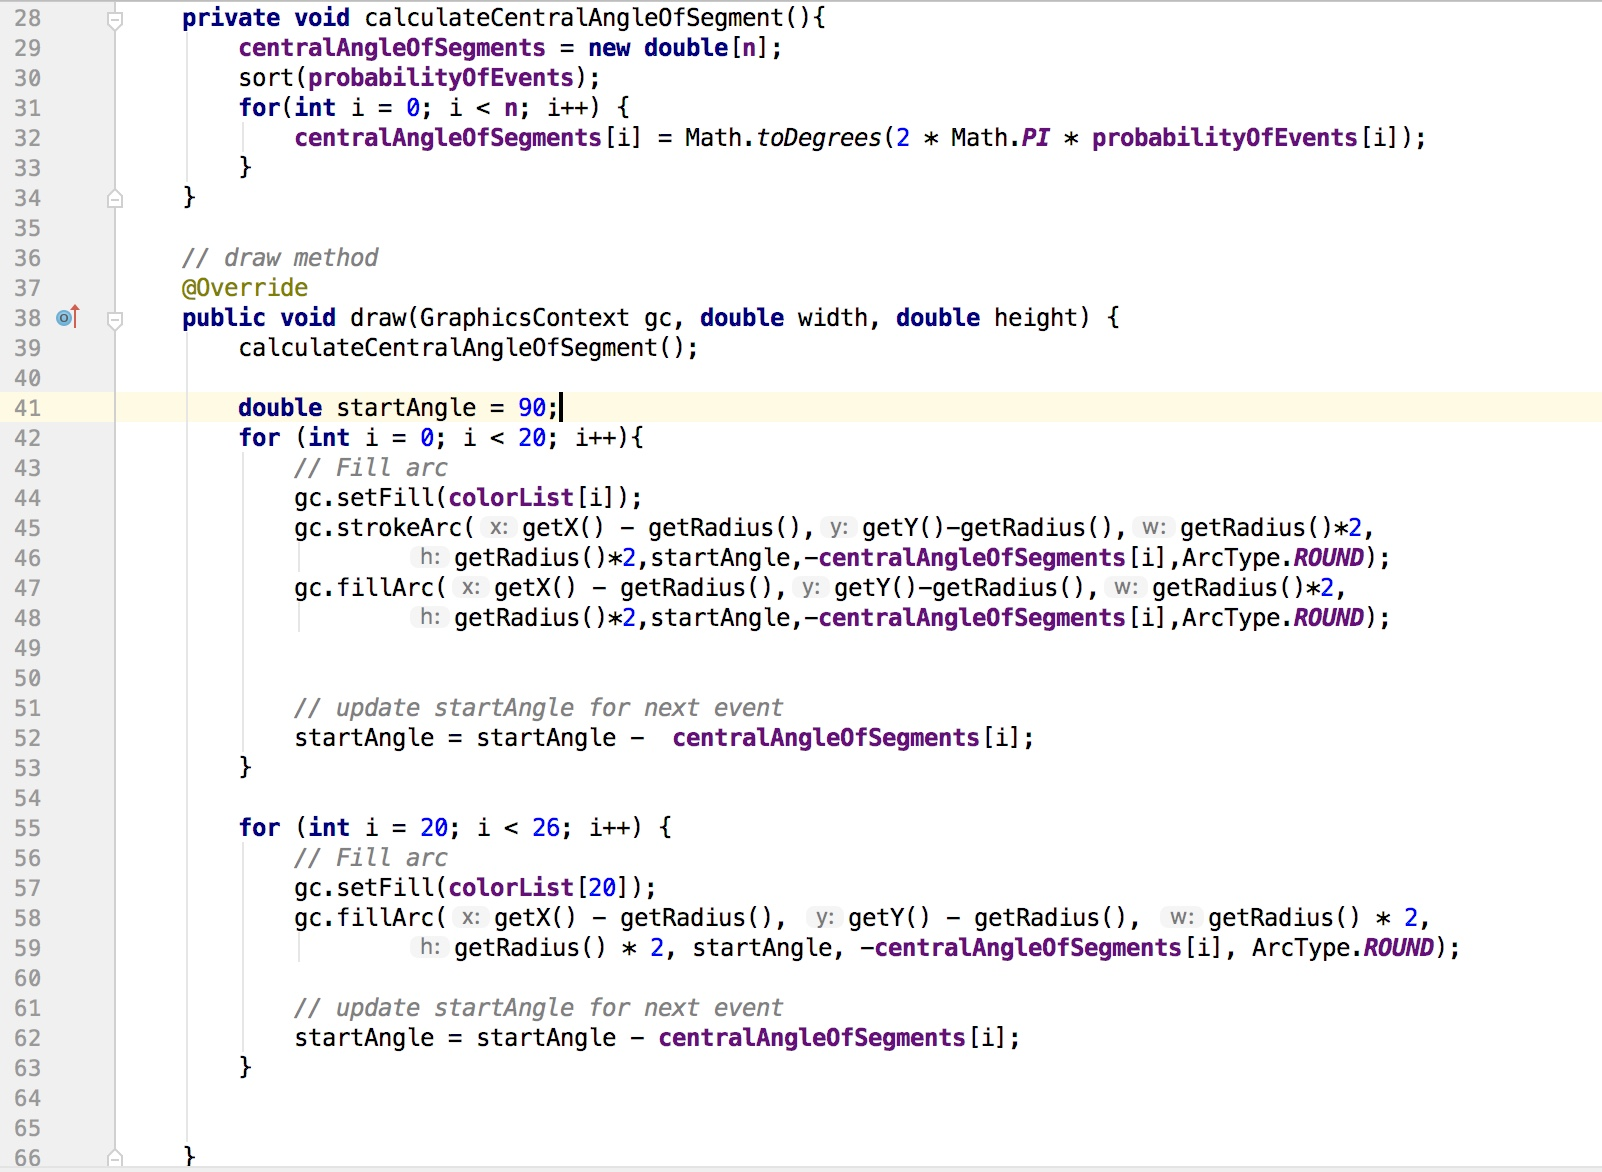
\includegraphics[width = 17cm]{pieChartPart2} % requires the graphicx package
   \caption{pieChartPart2}
   \label{pieChartPart2}
\end{figure}


\begin{figure}[H]
   \centering
   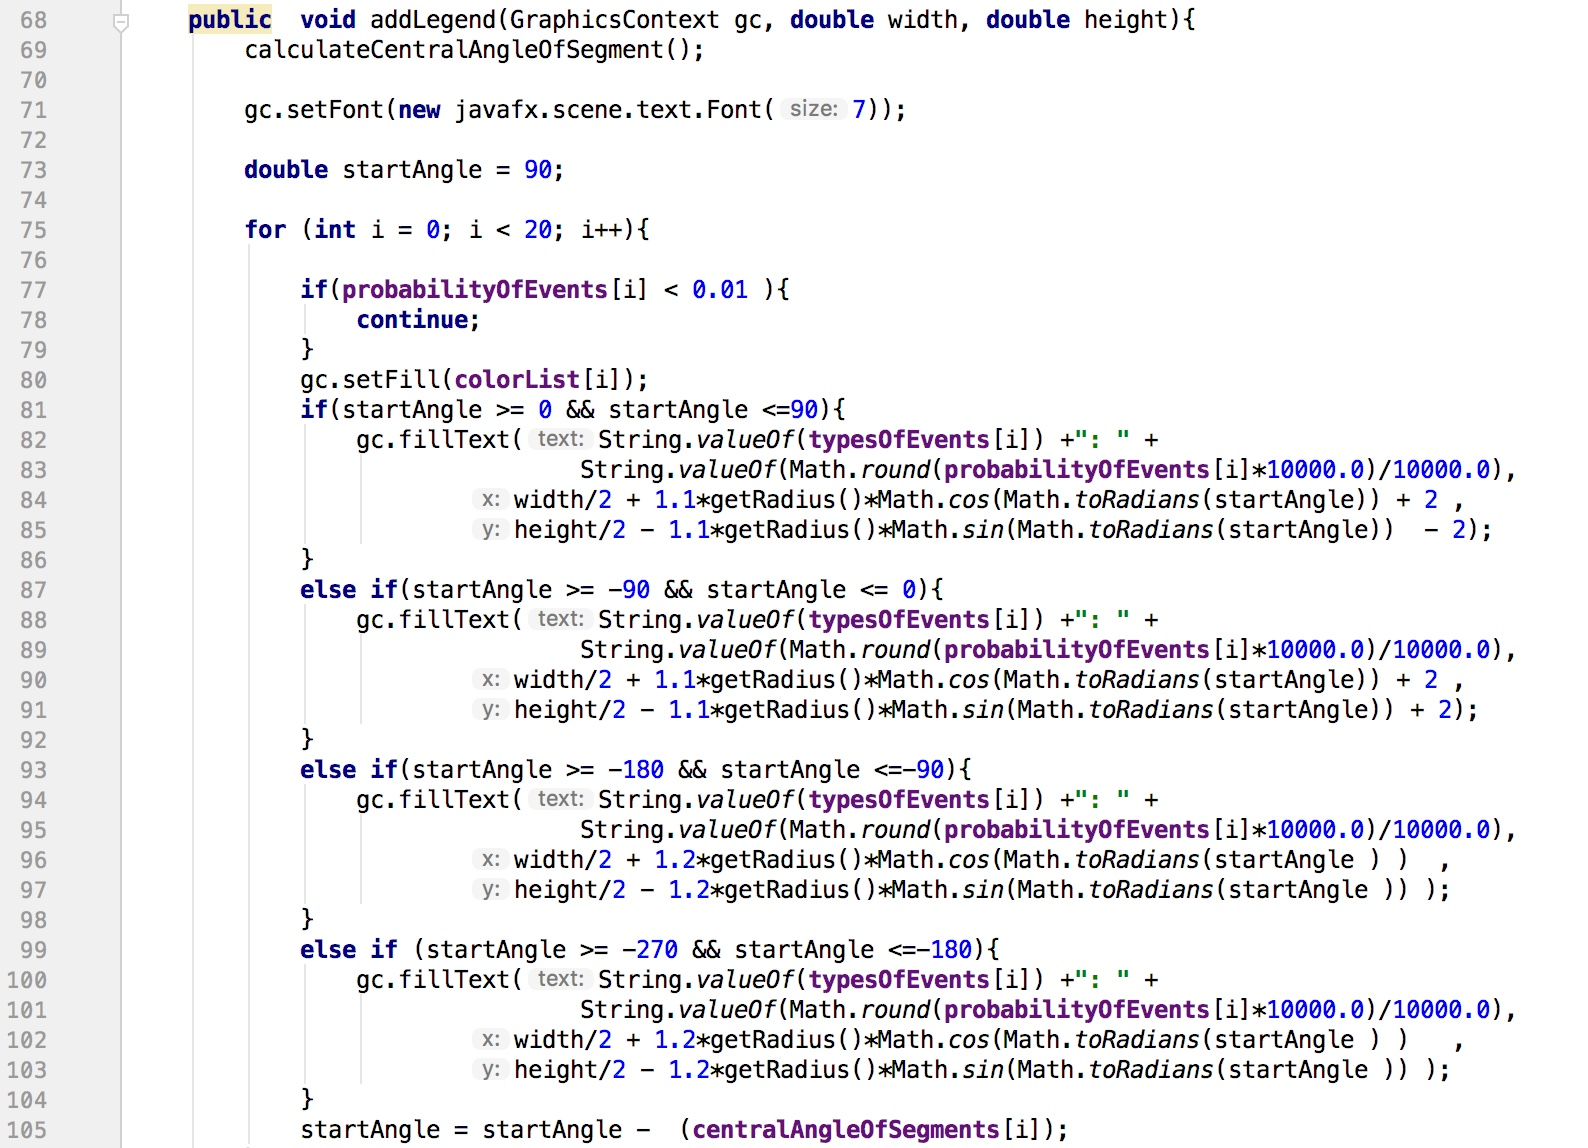
\includegraphics[width = 17cm]{pieChartPart3} % requires the graphicx package
   \caption{pieChartPart3}
   \label{pieChartPart3}
\end{figure}


\begin{figure}[H]
   \centering
   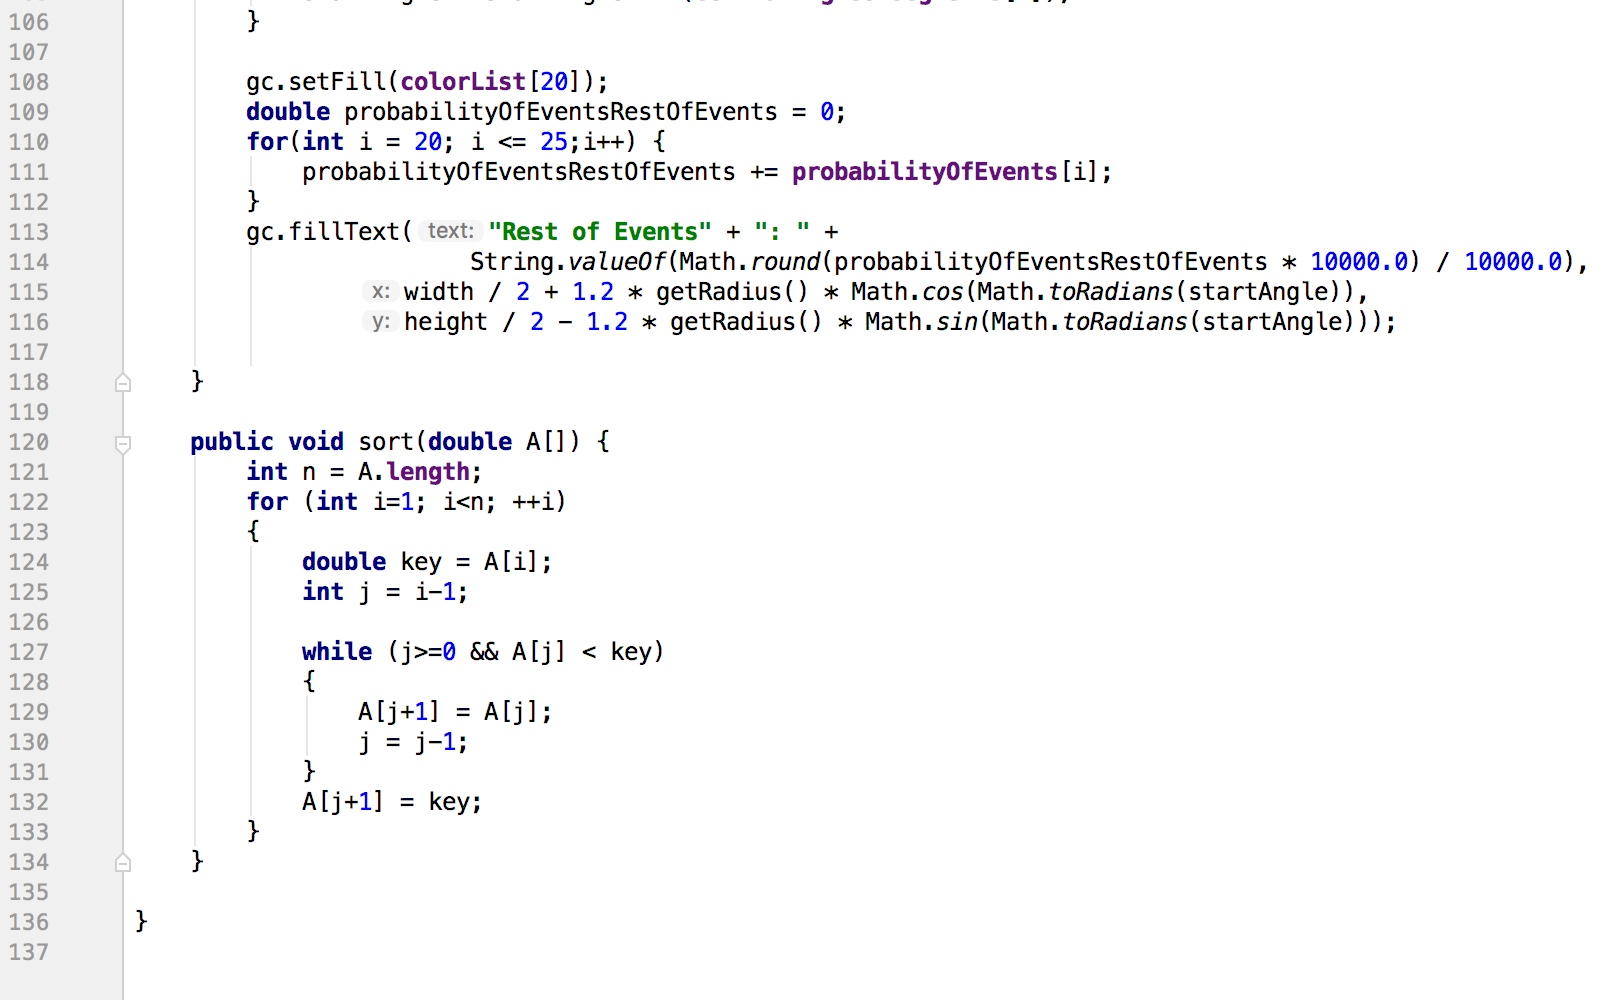
\includegraphics[width = 17cm]{pieChartPart4} % requires the graphicx package
   \caption{pieChartPart4}
   \label{pieChartPart4}
\end{figure}



\section{Part 2}


\subsection{Instructions}
The PieChart class includes appropriate constructors and a method draw that draws the pie chart. The drawing panel should include appropriate GUI components to input the number of events, n, and display the pie chart together with the events probabilities. You may amend and use the class hierarchy in previous exercises, but in any case you may only use your own classes and methods for the operations included.


\subsection{Solution Method}

As mentioned  previously, the Shape, and Circle classes are the super classes of PieChart. Figures \ref{shape1} - \ref{circle1} illustrate the code for both classes, including the declaration of their private members, constructors, set and get methods, as well as the toString and draw methods.  \newline

\vspace{0.25cm}
Two additional classes were required to incorporate the drawing panel with the GUI components. First, figures \ref{DrawPieChartControllerPart1} - \ref{DrawPieChartControllerPart2} shows the DrawPieChartController class which included all of the fxml components that allow the user to input the number of events to be drawn in the pie chat. The three components were the TextField numberEventsTextField which is used to obtain the value of n from the user, the canvas, where the shapes are drawn, and the drawShapesButtonPressed, which is the method with an ActionEvent as an arguments allowing the statements in its body to have any effect on the canvas. The rest of this class will be discussed in part 3.  Finally, the class DrawPieChart in figure \ref{DrawPieChartMain}  loads the PieChart.fxml file  and launches the application. 


\subsection{Code Developed}
\begin{figure}[H]
   \centering
   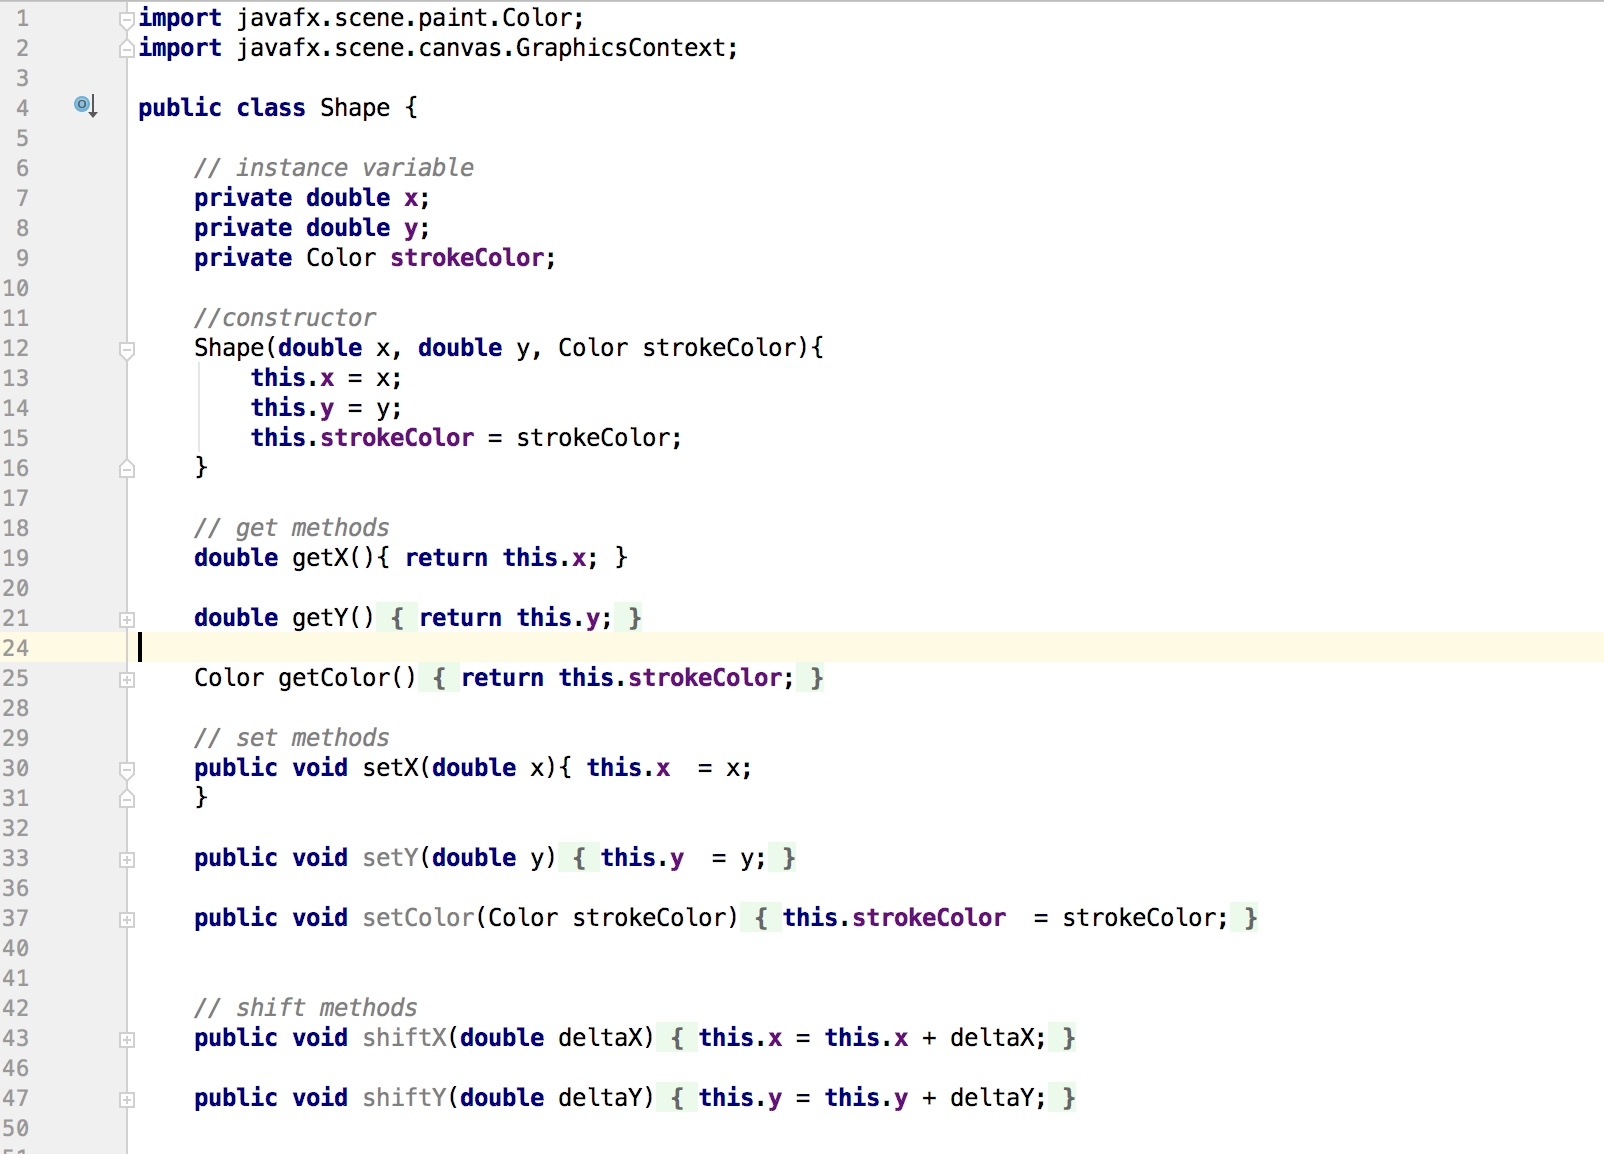
\includegraphics[width = 17cm]{shape1} % requires the graphicx package
   \caption{shape1}
   \label{shape1}
\end{figure}


\begin{figure}[H]
   \centering
   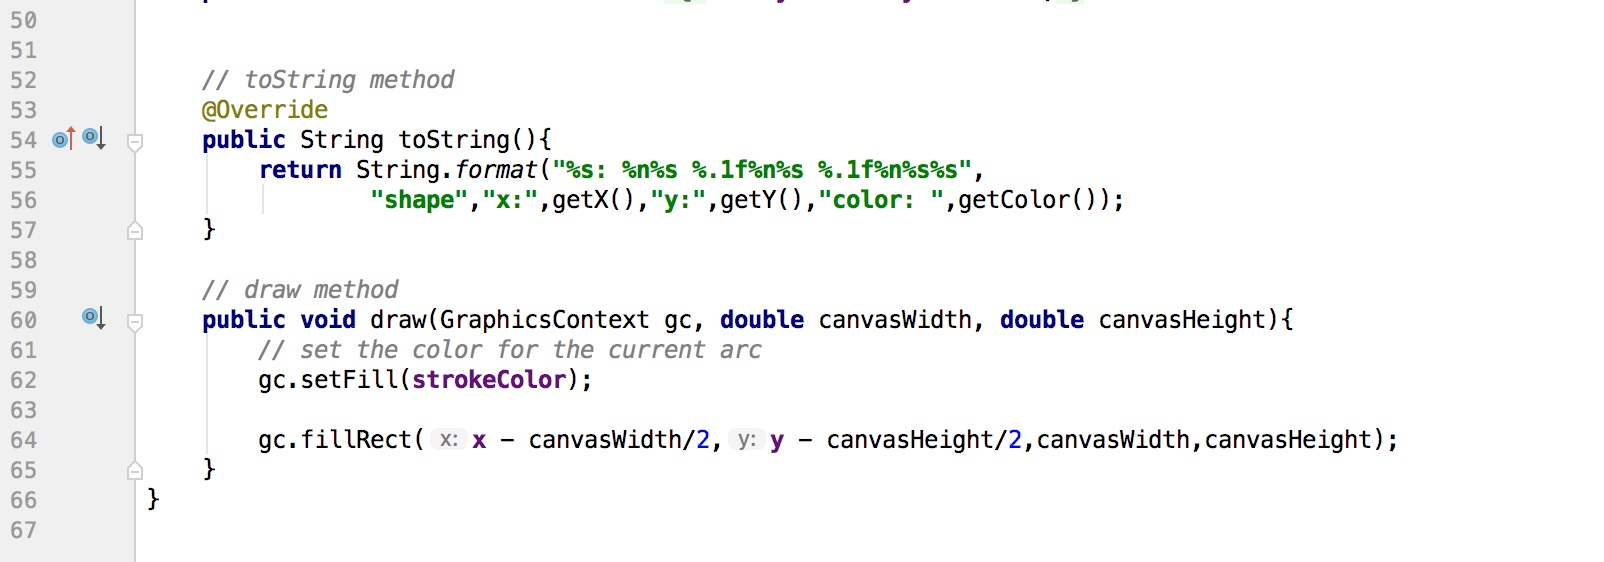
\includegraphics[width = 17cm]{shape2} % requires the graphicx package
   \caption{shape2}
   \label{shape2}
\end{figure}



\begin{figure}[H]
   \centering
   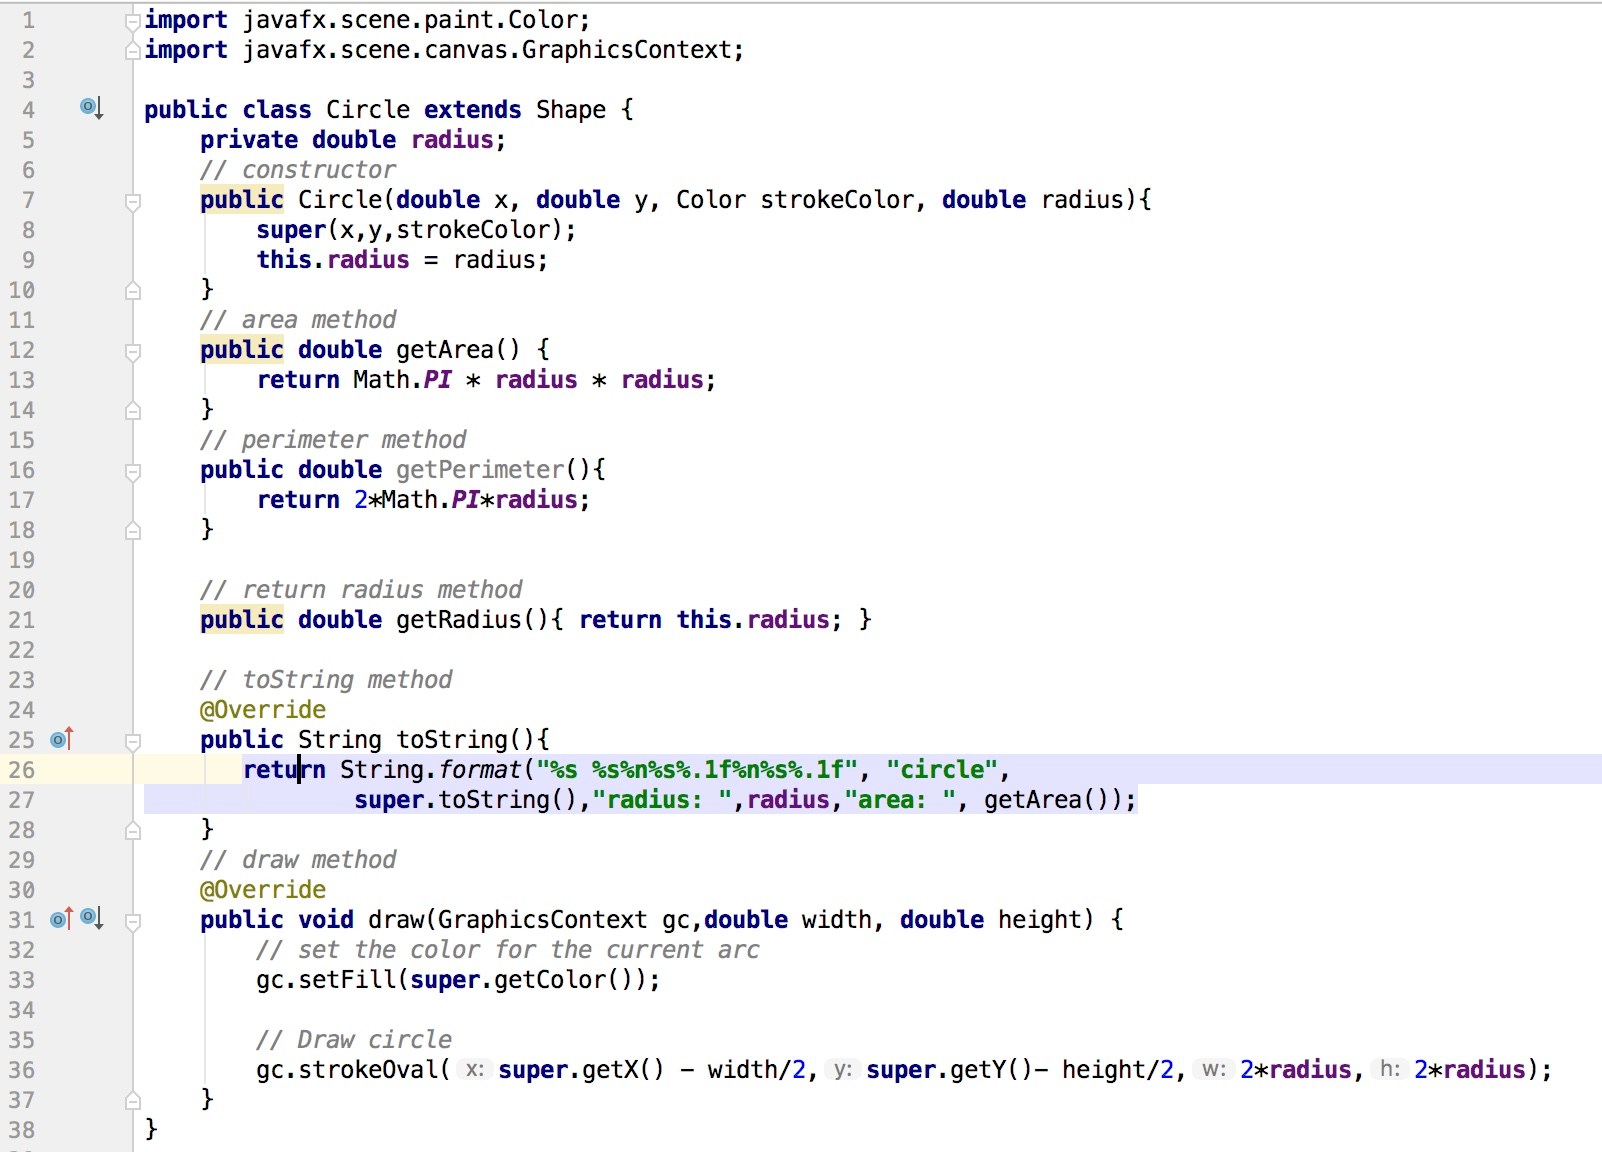
\includegraphics[width = 17cm]{circle1} % requires the graphicx package
   \caption{circle1}
   \label{circle1}
\end{figure}


\begin{figure}[H]
   \centering
   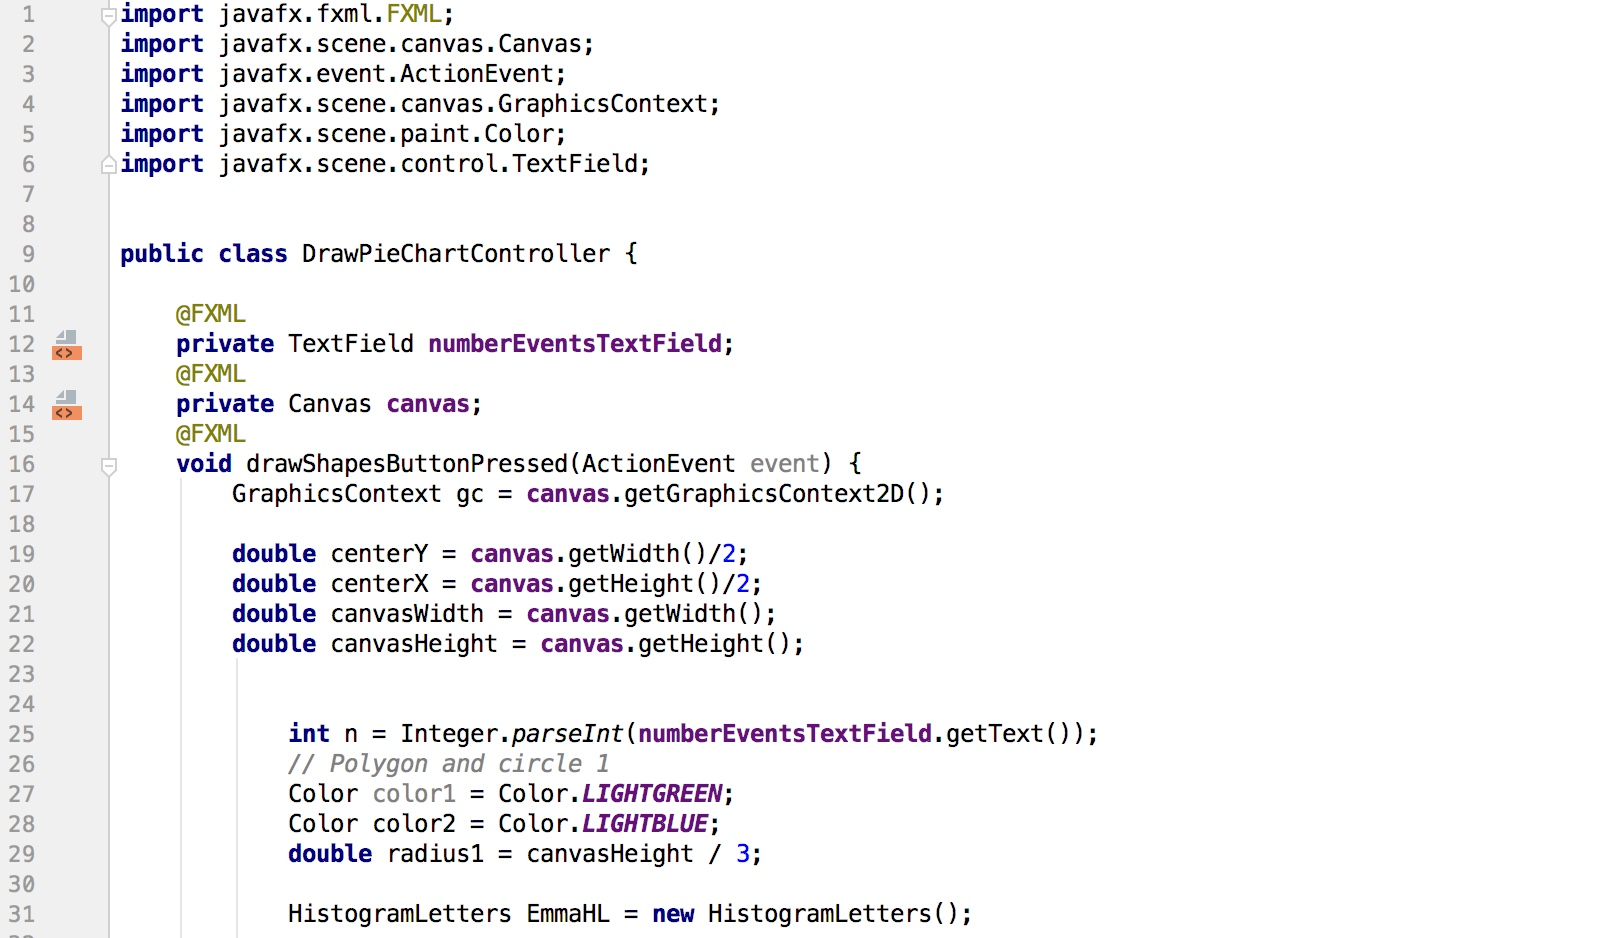
\includegraphics[width = 17cm]{DrawPieChartControllerPart1} % requires the graphicx package
   \caption{DrawPieChartControllerPart1}
   \label{DrawPieChartControllerPart1}
\end{figure}


\begin{figure}[H]
   \centering
   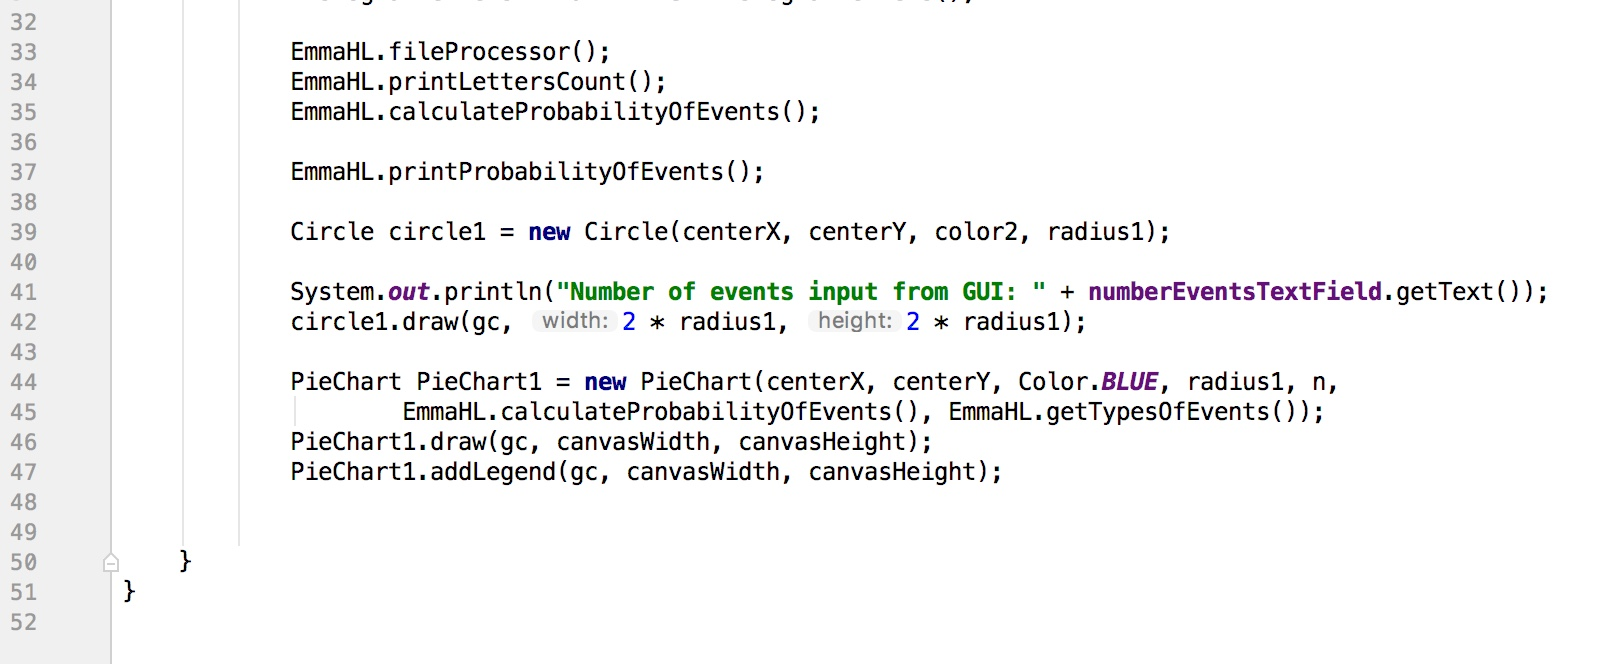
\includegraphics[width = 17cm]{DrawPieChartControllerPart2} % requires the graphicx package
   \caption{DrawPieChartControllerPart2}
   \label{DrawPieChartControllerPart2}
\end{figure}




\begin{figure}[H]
   \centering
   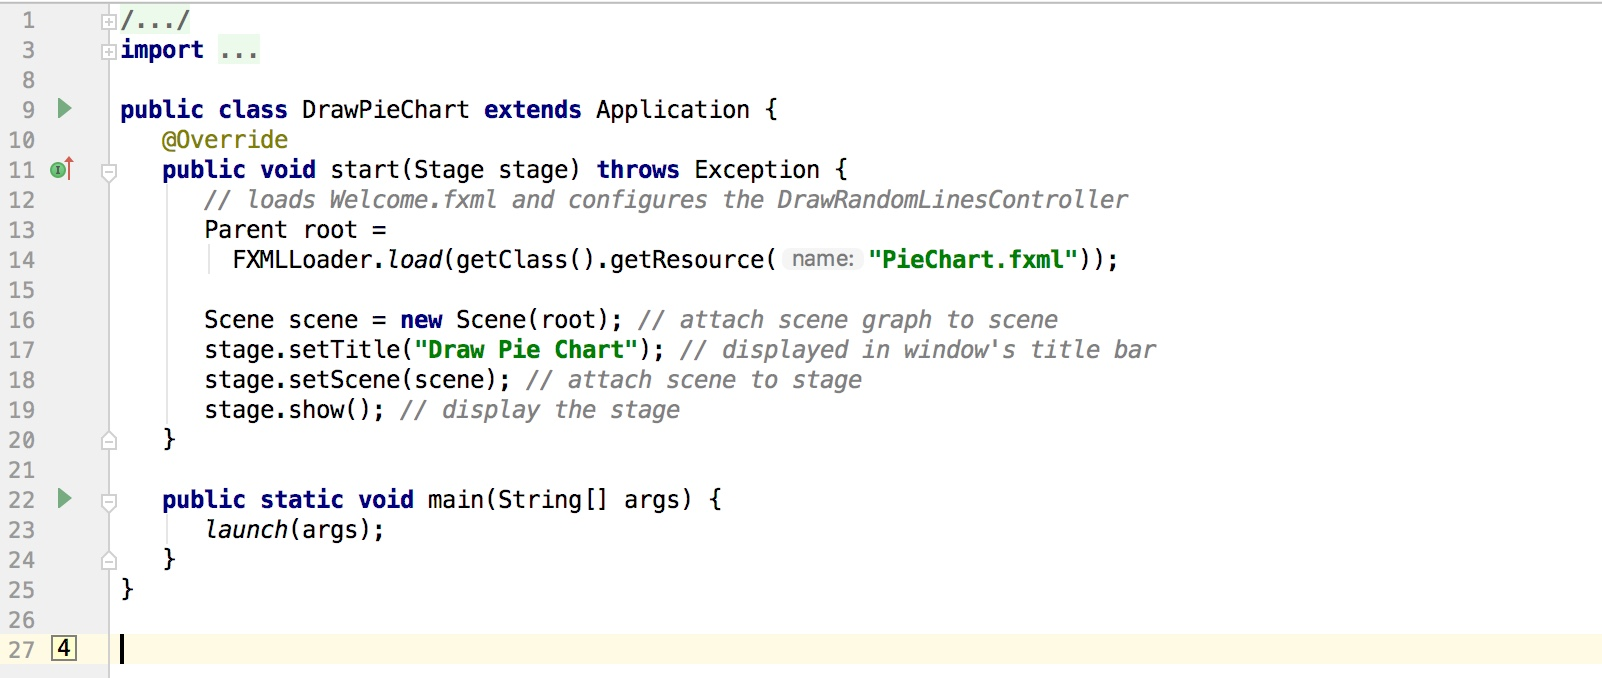
\includegraphics[width = 19cm]{DrawPieChart} % requires the graphicx package
   \caption{DrawPieChart}
   \label{DrawPieChartMain}
\end{figure}



\section{Part 3}

\subsection{Instructions}
 Implement a Java class HistogramLetters that calculates the n most frequent letters in the file ?Emma.txt? and their probabilities. The HistogramLetters class utilizes the drawing panel above to draw a pie chart of the letter probabilities.


\subsection{Solution Method}

The HistogramLetters class is shown in figures \ref{histogramLettersPart1} - \ref{histogramLettersPart3}. This class has the private members lettersCounter, probabilityOfEvents, and the englishAlphabet, and englishAlphabetCapital. The lettersCounter which is an array of integers representing the frequency of each letter in the book "Emma", and the probabilityOfEvents is an array of doubles with the probability of each letter calculated with the method getFrequencyOfAllEvents. \newline

\vspace{0.25cm}
The method fileProcessor uses a  while loop to read the text file "Emma" character-by-character and employees the method identifyLetter which identifies a letter increments and increments it by 1. This process repeats itself until the end of the file. Methods printLettersCount and printProbabilityOfEvents are used to check the frequency and probability of each letter, respectively.  \newline


\vspace{0.25cm}
 Finally, the HistogramLetters is used to instantiate  an object "EmmaHL" in the DrawPieChartController class in figure \ref{DrawPieChartControllerPart2}, which calls the methods fileProcessor, printLettersCount, calculateProbabilityOfEvents, and PrintProbability of events to double check the accuracy of the program. EmmaHL is also used to pass the probability of each event and the types of events to an object of PieChart class. The object "PieChart1" is used to draw the PieChart illustrated in figure \ref{resultPieChart}.



\subsection{Code Developed}

\begin{figure}[H]
   \centering
   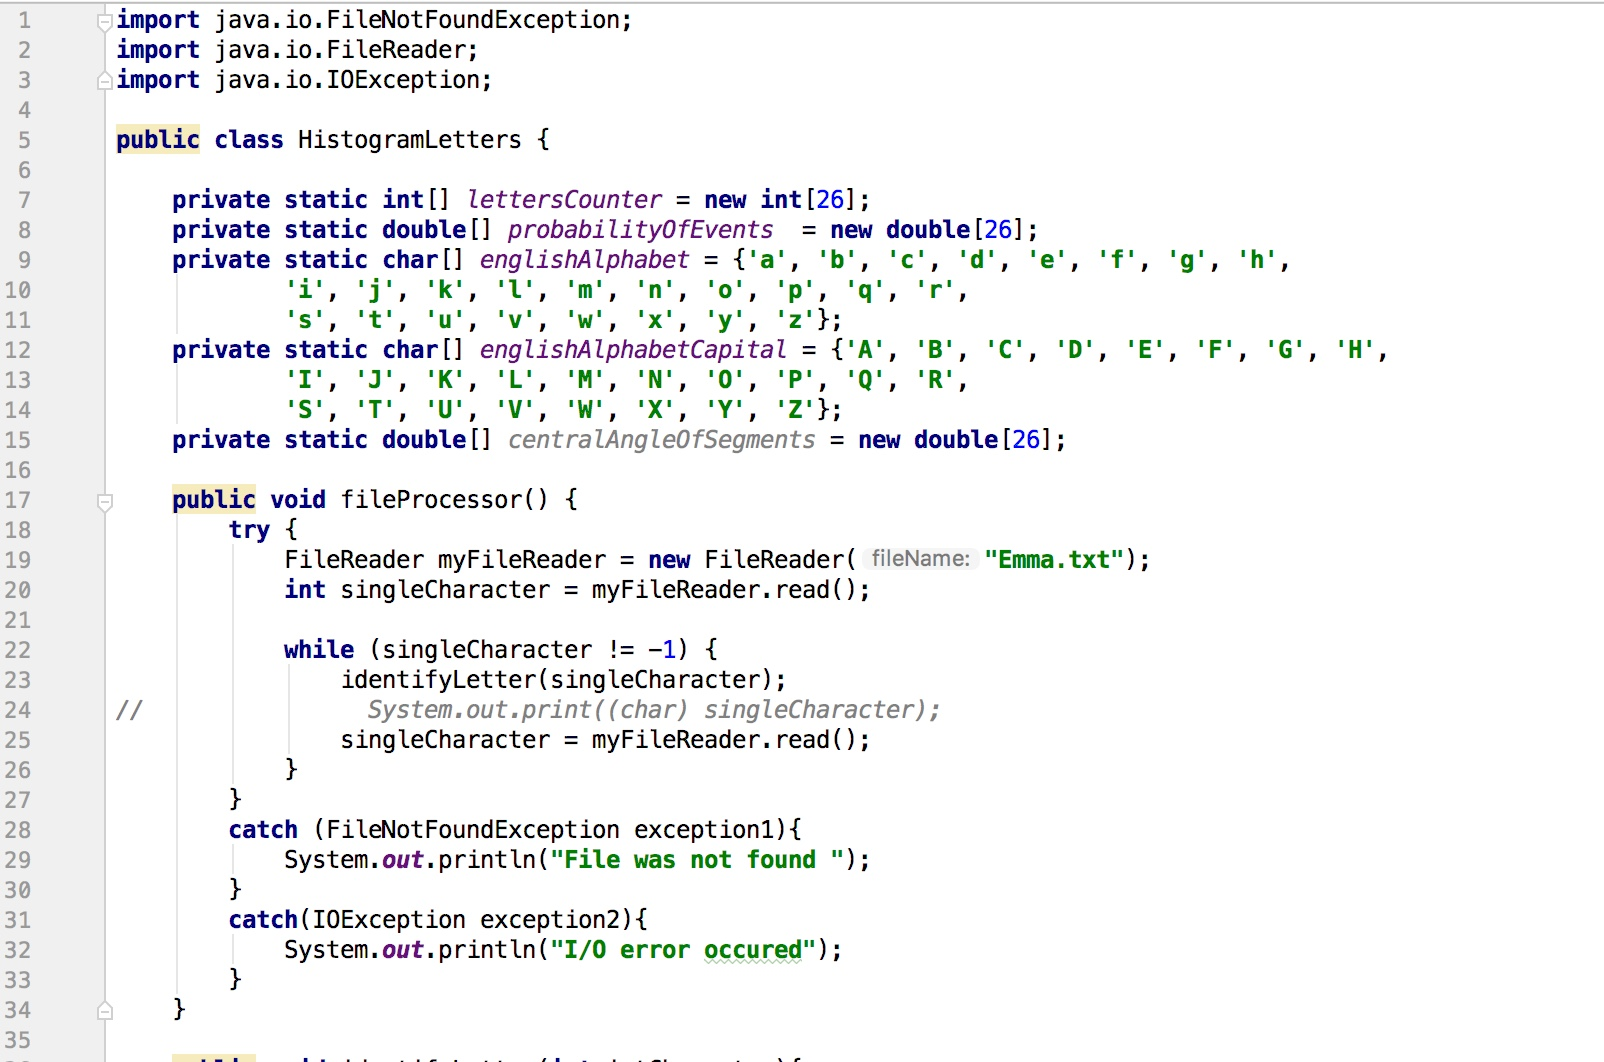
\includegraphics[width = 19cm]{histogramLettersPart1} % requires the graphicx package
   \caption{histogramLettersPart1}
   \label{histogramLettersPart1}
\end{figure}

\begin{figure}[H]
   \centering
   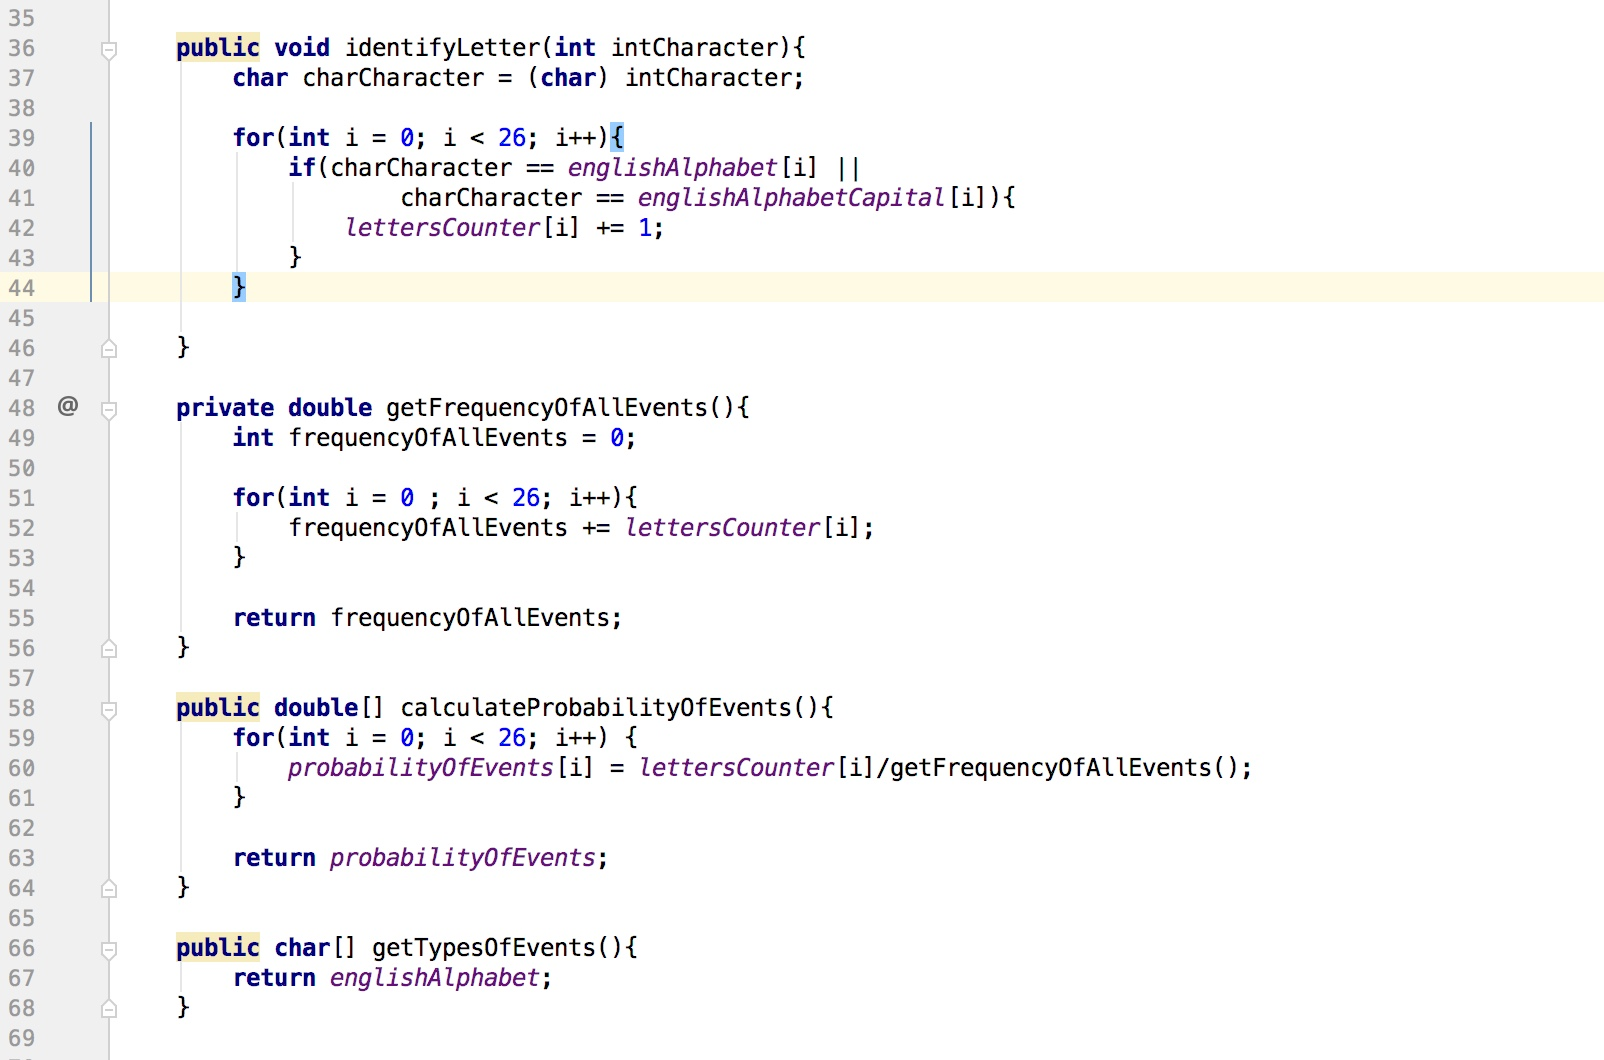
\includegraphics[width = 19cm]{histogramLettersPart2} % requires the graphicx package
   \caption{histogramLettersPart2t}
   \label{histogramLettersPart2}
\end{figure}

\begin{figure}[H]
   \centering
   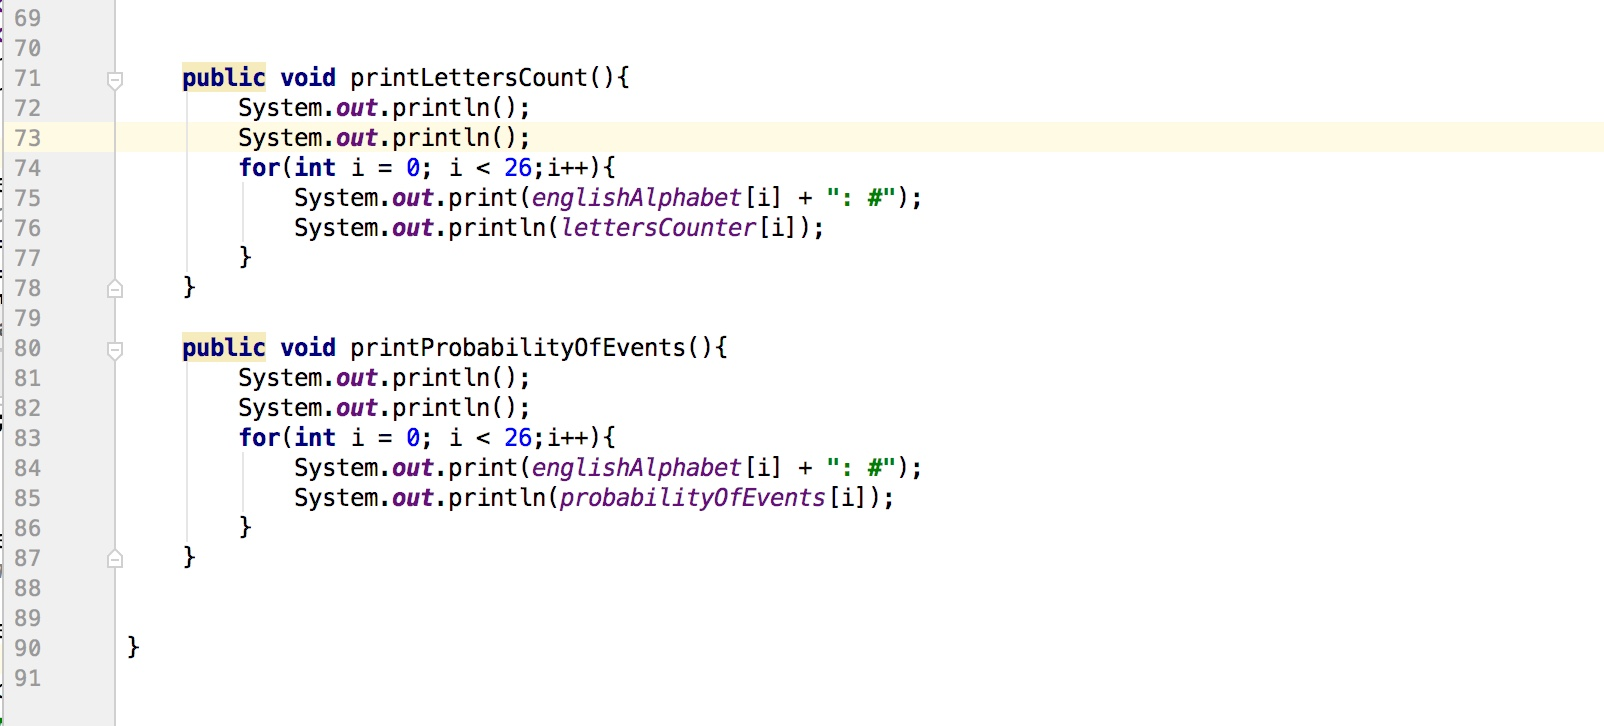
\includegraphics[width = 19cm]{histogramLettersPart3} % requires the graphicx package
   \caption{histogramLettersPart3}
   \label{histogramLettersPart3}
\end{figure}

\section{Results}



\subsection{Pie Chart for letters of Emma Book}

Figures \ref{resultPieChart} , \ref{Number of Repetition of each letter} , and \ref{OutputProbabilities} show the output results for the pieChart, the number of frequencies and probabilities of each events, respectively. The output pie chart for the histogram of Emma book in figure \ref{resultPieChart} shows the probability of the letters in this book. They are alphabetically order in the clockwise direction, starting with the probability for the letter a 90 degrees and finishing with the probability for the letter t, the rest probability for the rest of letters are represented in the region with the legend "Rest of Events: 0.0905. 

\begin{figure}[H]
   \centering
   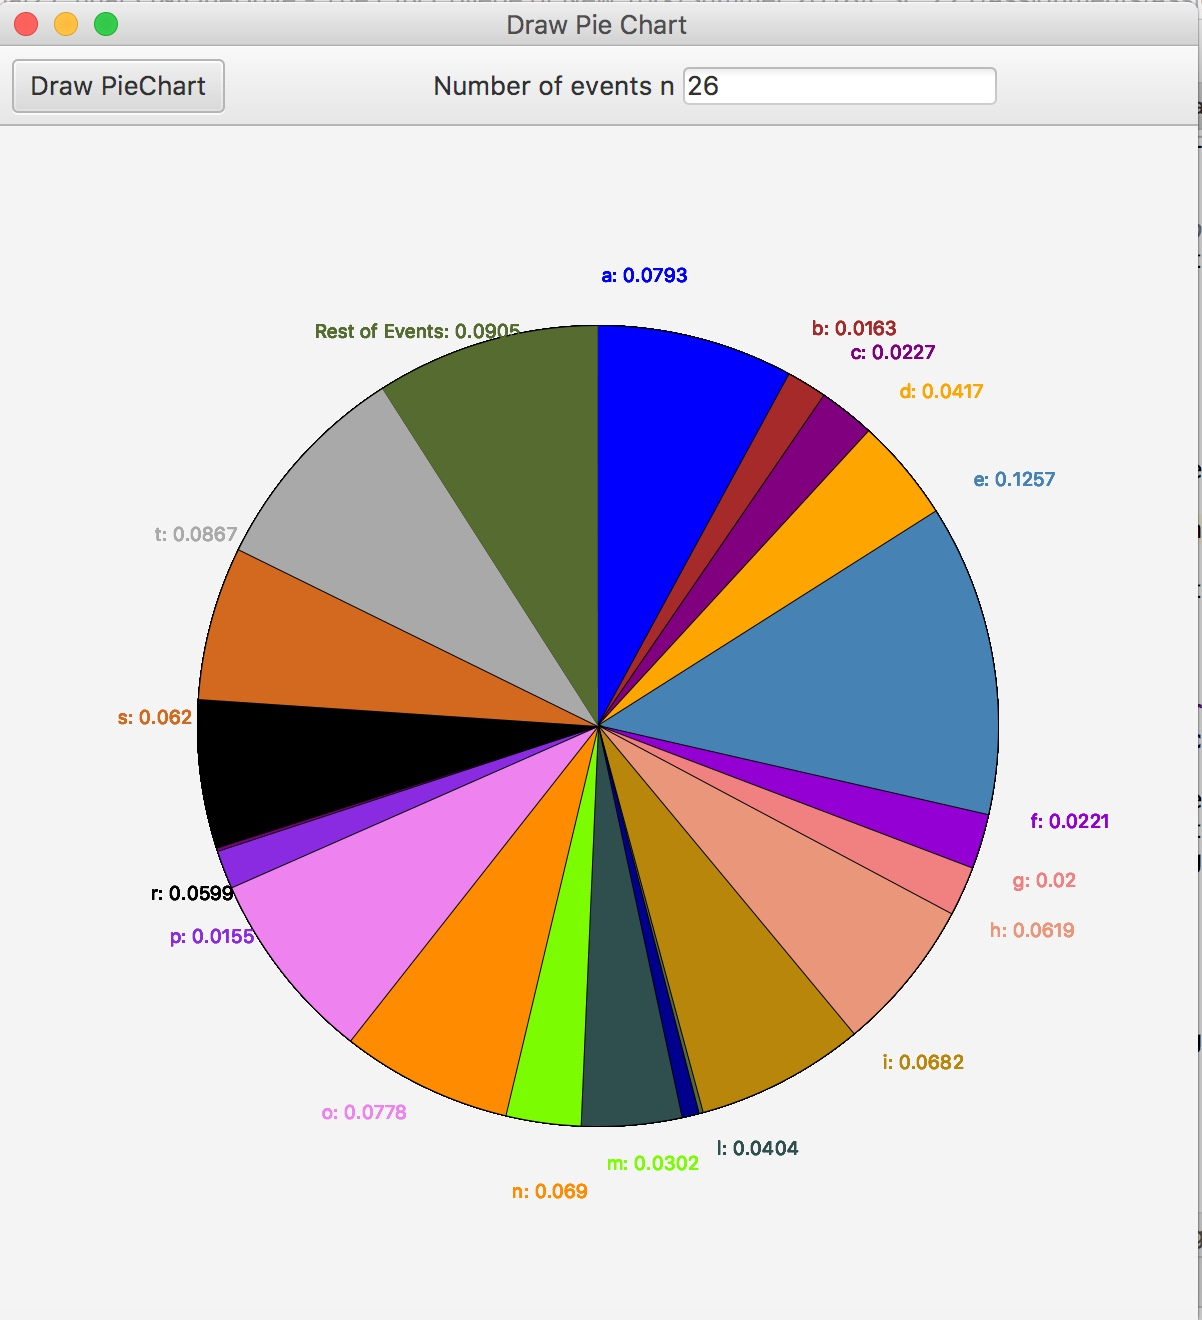
\includegraphics[width = 18cm]{resultPieChart} % requires the graphicx package
   \caption{resultPieChart}
   \label{resultPieChart}
\end{figure}

\subsection{Output for letters of Emma Book}

The frequency for each of the letters of the english alphabet in the book Emma are shown in figure  \ref{Number of Repetition of each letter}, this was the output from the program when the Histogram method printLettersCount() was used. 


\begin{figure}[H]
   \centering
   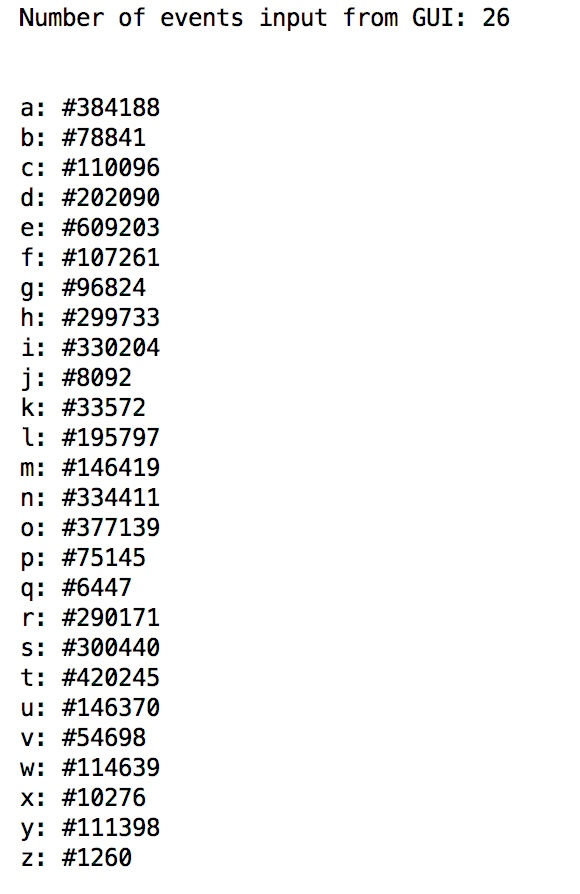
\includegraphics[width = 10cm]{outputFrequencies} % requires the graphicx package
   \caption{Number of Repetition of each letter}
   \label{Number of Repetition of each letter}
\end{figure}

\subsection{Output for possibilities of letters  of Emma Book}

The possibility for each of the letters of the english alphabet in the book Emma are shown in figure \ref{OutputProbabilities} , this was the output from the program when the Histogram method printProbabilityOfEvents was used. As one can observe, these probability values are indeed the same than the ones presented in the PieChart, showing the correctness of he addLegend() methods of the PieChart class. 


\begin{figure}[H]
   \centering
   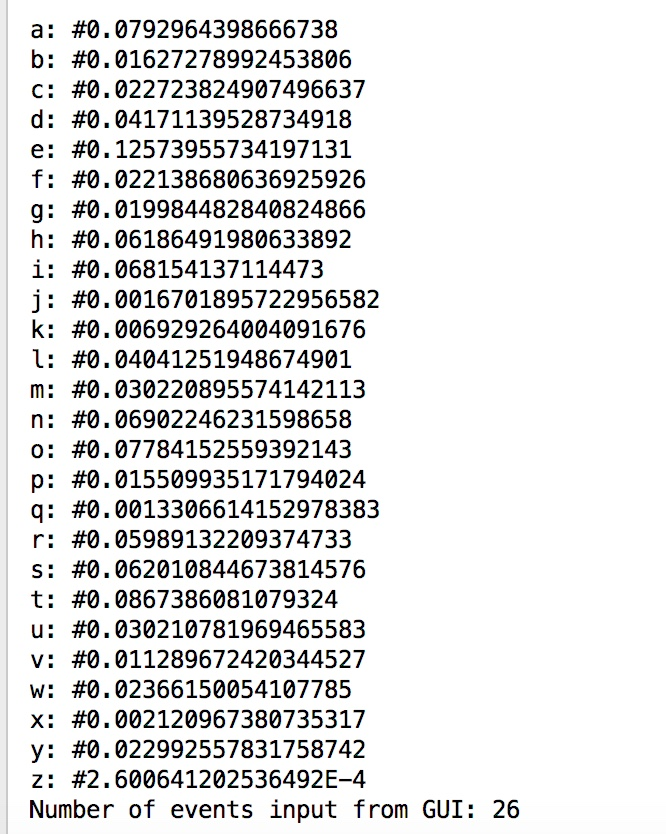
\includegraphics[width = 10cm]{OutputProbabilities} % requires the graphicx package
   \caption{Probabilities of each Letter}
   \label{OutputProbabilities}
\end{figure}




% ==========% ==========% ==========% ==========% ==========
\newpage
\section{References}
[1]  Deitel, Paul J., and Harvey M. Deitel. Java: How to Program Early Objects. Pearson, 2018.
\end{document}